\documentclass[11pt,a4paper]{article}
\usepackage[utf8]{inputenc}
\usepackage[T1]{fontenc}
\usepackage[margin=2.5cm]{geometry}
\usepackage{amsmath,amssymb}
\usepackage{graphicx}
\usepackage{booktabs}
\usepackage{siunitx}
\usepackage{microtype}
\usepackage{float}
\usepackage{xcolor}
\usepackage[font=small,labelfont=bf]{caption}
\usepackage[authoryear,round]{natbib}
\usepackage[colorlinks=true,linkcolor=blue!50!black,citecolor=blue!50!black,urlcolor=blue!50!black]{hyperref}
\usepackage[capitalise,noabbrev]{cleveref}

\graphicspath{{../figures/}}

\title{Market Risk of a Commodity Inventory:\\ VaR and Expected Shortfall Four Ways}
\author{Juan Carlos Chavarr\'ia Morales\\[2pt]
  \small M.Sc.\ Optimization, Hochschule Bielefeld (HSBI)\\
  \small Module \emph{Risikomanagement}, winter term 2024/25}
\date{October 2026}

\begin{document}
\maketitle

\begin{abstract}
A German company holds 500 tonnes of silver. Silver is priced in US dollars, the company reports in euros: the
euro value of the stock moves with the silver price and with the exchange rate. We measure the one-day 95\% Value
at Risk (VaR) of this exposure from one year of daily data (November 2022 to November 2023), extend it to a book of
silver and copper, and compare five methods: parametric (delta-normal), historical simulation, Monte Carlo with
normal and Student-$t$ shocks, and filtered historical simulation with EWMA volatility. The VaR of the silver stock
(EUR 334\,m) is EUR 8.3\,m, i.e.\ \SI{2.5}{\percent} of its value; ignoring the correlation between silver and the
dollar would overstate it by \SI{18}{\percent}, because the two act as a natural hedge in euros. For the two-commodity
book the one-day estimates of the methods differ by at most \SI{18}{\percent} and differ most in the tail (99\% ES, ten
days). All methods pass an out-of-sample backtest on the course data, but half a year of backtest has little power: a
99\% model with twice the nominal exception rate is rejected only one time in eight. On eleven years of public data
(2016--2026) the backtest separates the methods: the VaRs with normal tails are exceeded almost twice as often as
they should be at 99\%, and only historical and filtered historical simulation pass, the latter with the best
coverage.
\end{abstract}

% =====================================================================================================================
\section{The exposure}

Let $q_i$ be the quantity of commodity $i$ (in the unit of its price), $S_i$ its price in USD and $x$ the EUR/USD
rate (USD per EUR). The euro value of the book is
\begin{equation}
  V = \sum_i V_i, \qquad V_i = \frac{q_i S_i}{x}.
\end{equation}
With the risk factors $s_i = \log S_i$ and $f = \log x$, a scenario of factor changes $(\Delta s, \Delta f)$
revalues the book exactly (\emph{full revaluation}) as
\begin{equation}
  \Delta V = \sum_i V_i \left( e^{\Delta s_i - \Delta f} - 1 \right) \approx \sum_i V_i(\Delta s_i - \Delta f),
\end{equation}
the right-hand side being the delta approximation. A rise of the dollar ($\Delta f < 0$) raises the euro value; when
silver and the euro rise together, the two effects cancel. The loss is $L = -\Delta V$; for a level $\alpha$,
$\mathrm{VaR}_\alpha$ is the $\alpha$-quantile of $L$ and the expected shortfall
$\mathrm{ES}_\alpha = \mathbb E[L \mid L \ge \mathrm{VaR}_\alpha]$ the mean loss beyond it \citep{McNeil2015}. ES is a
coherent risk measure \citep{Artzner1999}; VaR is not, but remains the reference in reporting.

\paragraph{The case.} The course exercise gives 500\,t of silver (\num{16.1e6} troy ounces) and asks for the one-day
VaR(95\%) of its euro value, ``taking into account the correlation that follows from the data''. As a second
position we add 40\,000\,t of copper; the course gives no quantity, so it is chosen to make the two positions of
similar size (EUR 334\,m and EUR 300\,m on 10 November 2023).

\paragraph{Data.} Daily closes of silver (USD/oz), copper (USD/t) and EUR/USD from 2 November 2022 to 10 November
2023, as provided in the course (source: finanzen.net). Silver and EUR/USD also contain weekend quotes; on the 258
weekdays on which all three closed we have 257 daily returns (\cref{fig:prices}). Annualised volatilities are
\SI{27}{\percent} (silver), \SI{20}{\percent} (copper) and \SI{9}{\percent} (EUR/USD); silver correlates with EUR/USD
at $+0.48$ and with copper at $+0.21$. All three return series have excess kurtosis (2.2, 1.4 and 0.7): fat tails,
one of the stylised facts of financial returns. The course data are not redistributed; the repository contains a
script that builds the same table from public sources \citep{Repo}.

\begin{figure}[t]
  \centering
  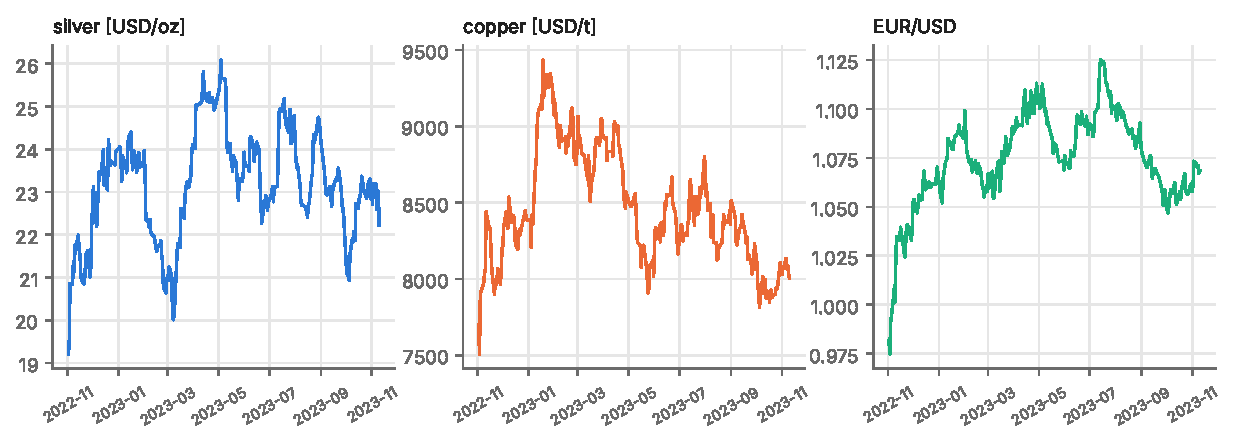
\includegraphics[width=\linewidth]{prices.pdf}
  \caption{Daily closes used in the study (weekdays common to the three series).}
  \label{fig:prices}
\end{figure}

% =====================================================================================================================
\section{Methods}

\begin{description}
  \item[Parametric (delta-normal).] Factor changes normal with the sample covariance $\Sigma$, delta approximation:
    $L \sim N(0, \delta^\top \Sigma \delta)$ with $\delta = (V_1, \dots, V_n, -V)$, so
    $\mathrm{VaR}_\alpha = z_\alpha \sigma_L$ and $\mathrm{ES}_\alpha = \sigma_L \varphi(z_\alpha)/(1-\alpha)$.
  \item[Historical simulation.] Today's book revalued under every observed (overlapping) $h$-day factor change; no
    distributional assumption, but only as many scenarios as days.
  \item[Monte Carlo.] \num{200000} correlated scenarios (Cholesky factor of $\Sigma$) with full revaluation, with
    normal shocks or multivariate Student-$t$ shocks of the same covariance; the degrees of freedom ($\nu = 8.2$) are
    fitted to the daily P\&L of the book.
  \item[Filtered historical simulation.] Each factor's returns are divided by their EWMA volatility
    ($\lambda = 0.94$, \citealp{RiskMetrics1996}) and rescaled by today's forecast \citep{HullWhite1998}: the
    empirical joint shape of the shocks is kept, volatility clustering is taken into account.
\end{description}
For ten days, the parametric and Monte Carlo methods scale the covariance by 10 (square-root-of-time); the
historical methods use overlapping ten-day returns. Risk contributions follow the Euler allocation of the
parametric VaR, $C_i = z_\alpha \operatorname{cov}(L_i, L)/\sigma_L$, which adds up to the VaR of the book
\citep{Tasche1999}.

% =====================================================================================================================
\section{The course exercise: 500 t of silver}

The one-day VaR(95\%) of the silver stock is \textbf{EUR 8.28\,m}, \SI{2.5}{\percent} of its value of EUR 334\,m;
the ES(95\%) is EUR 10.4\,m. The exercise asked for the correlation, and it matters: with the same volatilities
and zero correlation, the VaR would be EUR 9.76\,m, \SI{18}{\percent} higher. Silver and the euro tend to rise
together against the dollar ($\rho = +0.48$), so part of a fall of silver in USD is offset in EUR by a weaker euro and
vice versa: holding silver in a euro balance sheet is less risky than its dollar volatility suggests (silver price
risk alone: EUR 9.29\,m).

% =====================================================================================================================
\section{The book: silver and copper}\label{sec:book}

\Cref{tab:var} compares the methods. At the one-day horizon and 95\%, they differ by at most \SI{18}{\percent}
(EUR 8.8--10.4\,m); the filtered historical simulation is lowest because volatility at the end of the sample was
below its one-year average. At 99\% and ten days the differences grow: the Student-$t$ Monte Carlo and the filtered
historical simulation have the largest ES (EUR 57--59\,m), the plain historical simulation the smallest, because 248
overlapping ten-day returns contain few independent extreme scenarios. \Cref{fig:loss} shows the historical loss
distribution of today's book with the five one-day VaR estimates.

\begin{table}[t]
  \centering\small
  \caption{VaR and ES of the silver and copper book (EUR m), as of 10 November 2023.}
  \label{tab:var}
  \resizebox{\linewidth}{!}{\begin{tabular}{lrrrrrrrr}
\toprule
& \multicolumn{4}{c}{95\%} & \multicolumn{4}{c}{99\%} \\ \cmidrule(lr){2-5}\cmidrule(lr){6-9}& \multicolumn{2}{c}{1 day} & \multicolumn{2}{c}{10 days} & \multicolumn{2}{c}{1 day} & \multicolumn{2}{c}{10 days} \\
method & VaR & ES & VaR & ES & VaR & ES & VaR & ES \\
\midrule
parametric (delta-normal) & 10.4 & 13.1 & 33.0 & 41.4 & 14.7 & 16.9 & 46.6 & 53.4 \\
historical simulation & 9.8 & 12.4 & 30.2 & 35.0 & 14.7 & 16.2 & 39.4 & 41.2 \\
Monte Carlo, normal & 10.3 & 12.9 & 31.8 & 39.7 & 14.6 & 16.7 & 44.7 & 51.0 \\
Monte Carlo, Student t & 10.1 & 13.6 & 31.1 & 41.6 & 15.7 & 19.4 & 47.9 & 58.8 \\
filtered HS (EWMA) & 8.8 & 13.1 & 27.4 & 39.7 & 14.7 & 19.0 & 45.4 & 57.4 \\
\bottomrule
\end{tabular}
}
\end{table}

\begin{figure}[t]
  \centering
  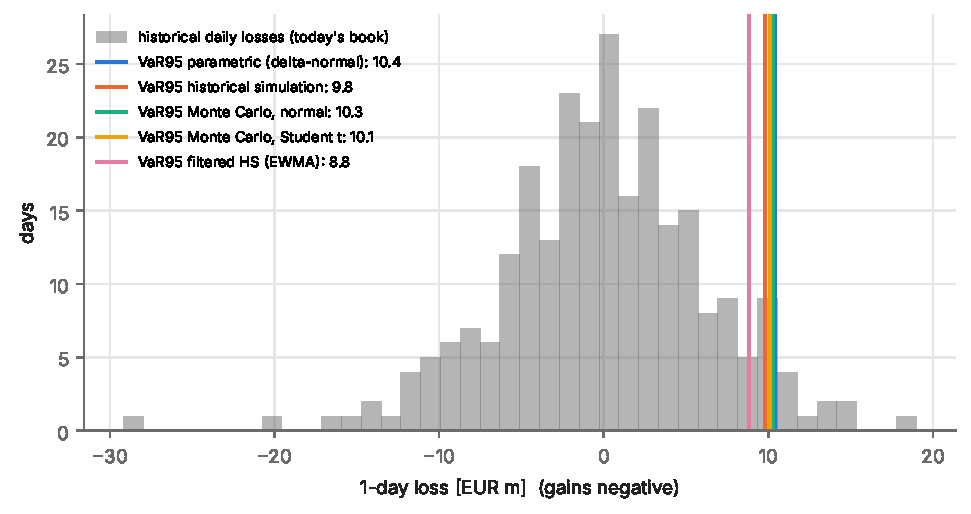
\includegraphics[width=0.85\linewidth]{loss_distribution.pdf}
  \caption{One-day losses of today's book under the 257 historical scenarios, and the one-day VaR(95\%) of the five
    methods.}
  \label{fig:loss}
\end{figure}

\paragraph{Diversification.} The stand-alone VaRs of silver and copper add up to EUR 14.2\,m; the VaR of the book
is EUR 10.4\,m, \SI{27}{\percent} less (\cref{tab:contrib,fig:div}). Silver contributes two thirds of the book VaR
for a little over half of its value: copper is less volatile and only weakly correlated with silver.

\begin{table}[H]
  \centering\small
  \caption{Euler allocation of the one-day parametric VaR(95\%) (EUR m).}
  \label{tab:contrib}
  \begin{tabular}{lrrr}
\toprule
position & value [EUR m] & stand-alone VaR & contribution \\
\midrule
silver & 334 & 8.28 & 6.82 \\
copper & 300 & 5.92 & 3.61 \\
\midrule book & 634 & 14.20 & 10.43 \\
\bottomrule
\end{tabular}

\end{table}

\begin{figure}[H]
  \centering
  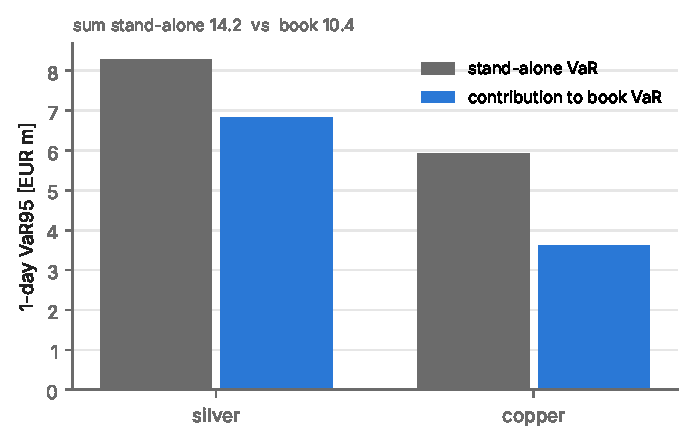
\includegraphics[width=0.55\linewidth]{diversification.pdf}
  \caption{Stand-alone VaR and contribution to the book VaR of each position.}
  \label{fig:div}
\end{figure}

% =====================================================================================================================
\section{Backtest}

Each day from May 2023, the one-day VaR is estimated from the previous 125 days and compared with the realised loss
of the book on the next day (132 days, \cref{fig:backtest}). The Kupiec test checks the number of exceptions
\citep{Kupiec1995}, the Christoffersen test their independence \citep{Christoffersen1998}. All methods pass both at
95\% and 99\% (\cref{tab:backtest}).

\begin{table}[t]
  \centering\small
  \caption{Out-of-sample backtest of the one-day VaR (rolling window of 125 days, 132 test days).}
  \label{tab:backtest}
  \begin{tabular}{lrrrrr}
\toprule
method & level & expected & exceptions & Kupiec $p$ & Christoffersen $p$ \\
\midrule
parametric (delta-normal) & 95\% & 6.6 & 5 & 0.51 & 0.62 \\
historical simulation & 95\% & 6.6 & 7 & 0.87 & 0.45 \\
Monte Carlo, normal & 95\% & 6.6 & 5 & 0.51 & 0.62 \\
filtered HS (EWMA) & 95\% & 6.6 & 7 & 0.87 & 0.45 \\
parametric (delta-normal) & 99\% & 1.3 & 2 & 0.58 & 0.80 \\
historical simulation & 99\% & 1.3 & 3 & 0.21 & 0.76 \\
Monte Carlo, normal & 99\% & 1.3 & 2 & 0.58 & 0.80 \\
filtered HS (EWMA) & 99\% & 1.3 & 3 & 0.21 & 0.76 \\
\bottomrule
\end{tabular}

\end{table}

\begin{figure}[t]
  \centering
  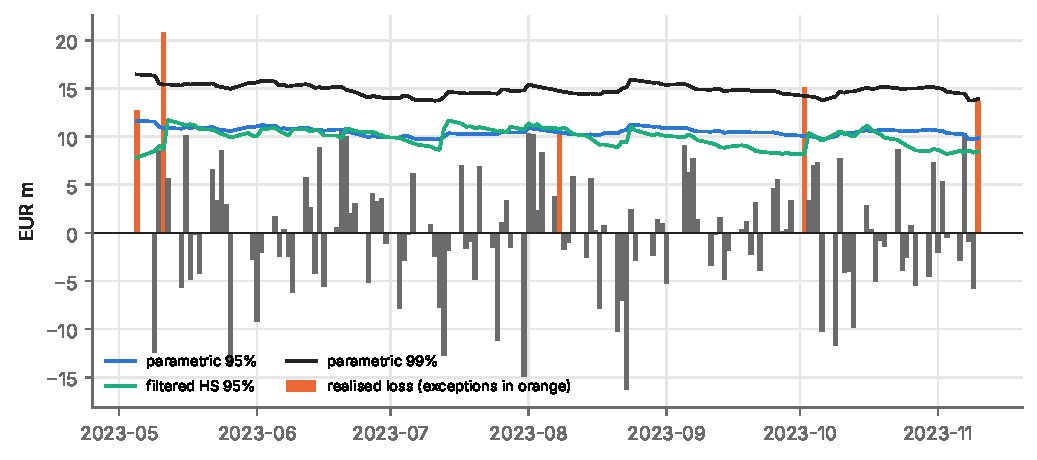
\includegraphics[width=0.9\linewidth]{backtest.pdf}
  \caption{Realised daily losses of the book (exceptions of the parametric 95\% VaR in orange) and the rolling VaR
    forecasts.}
  \label{fig:backtest}
\end{figure}

A passed backtest of this length is weak evidence. \Cref{tab:power} gives the probability that the Kupiec test
rejects a model whose true exception rate is too high: a 95\% VaR that is exceeded on \SI{10}{\percent} of the days
is caught in about half of the cases, a 99\% VaR exceeded on \SI{2}{\percent} of the days in one case out of eight.
Regulatory backtests use 250 days or more for this reason, and at the 99\% level even a year leaves little power.

\begin{table}[H]
  \centering\small
  \caption{Power of the Kupiec test with 132 backtest days (5\% significance).}
  \label{tab:power}
  \begin{tabular}{rrr}
\toprule
VaR level & true exception rate & probability of rejection \\
\midrule
95\% & 7.5\% & 19\% \\
95\% & 10.0\% & 57\% \\
95\% & 15.0\% & 97\% \\
99\% & 1.5\% & 5\% \\
99\% & 2.0\% & 13\% \\
99\% & 3.0\% & 36\% \\
\bottomrule
\end{tabular}

\end{table}

% =====================================================================================================================
\section{Backtest on eleven years of public data}\label{sec:public}

The course data cover one year. With \texttt{scripts/fetch\_data.py} the same book (the quantities of
\cref{sec:book} held constant) was backtested on public data: the ECB reference rate and front-month COMEX futures
for silver and copper (Yahoo Finance), 2 January 2015 to 16 October 2026. The VaR is estimated each day from the
previous 250 days, giving 2686 test days from January 2016 on. The prices are not redistributed; the repository
keeps the test statistics (\texttt{results/public\_snapshot}).

Over this period the returns are far from normal: the excess kurtosis of the daily log returns is 36 for silver and
27 for copper, and a multivariate Student-$t$ fit gives $\nu = 3.5$ degrees of freedom (8.2 on the course year). The
largest moves are single days: silver fell by \SI{31}{\percent} on 30 January 2026, copper by \SI{22}{\percent} on
31 July 2025, when the US exempted refined copper from its import tariff. Front-month futures also contain roll
effects; both make the tails heavier than in a spot series.

\begin{table}[t]
  \centering\small
  \caption{Out-of-sample backtest on public data (rolling window of 250 days, 2686 test days, 2016--2026).}
  \label{tab:backtest_public}
  \begin{tabular}{lrrrrr}
\toprule
method & level & expected & exceptions & Kupiec $p$ & Christoffersen $p$ \\
\midrule
parametric (delta-normal) & 95\% & 134.3 & 122 & 0.269 & 0.030 \\
historical simulation & 95\% & 134.3 & 147 & 0.268 & 0.294 \\
Monte Carlo, normal & 95\% & 134.3 & 127 & 0.514 & 0.053 \\
filtered HS (EWMA) & 95\% & 134.3 & 135 & 0.951 & 0.932 \\
parametric (delta-normal) & 99\% & 26.9 & 45 & 0.001 & 0.045 \\
historical simulation & 99\% & 26.9 & 35 & 0.132 & 0.085 \\
Monte Carlo, normal & 99\% & 26.9 & 48 & 0.000 & 0.064 \\
filtered HS (EWMA) & 99\% & 26.9 & 33 & 0.250 & 0.067 \\
\bottomrule
\end{tabular}

\end{table}

\begin{figure}[t]
  \centering
  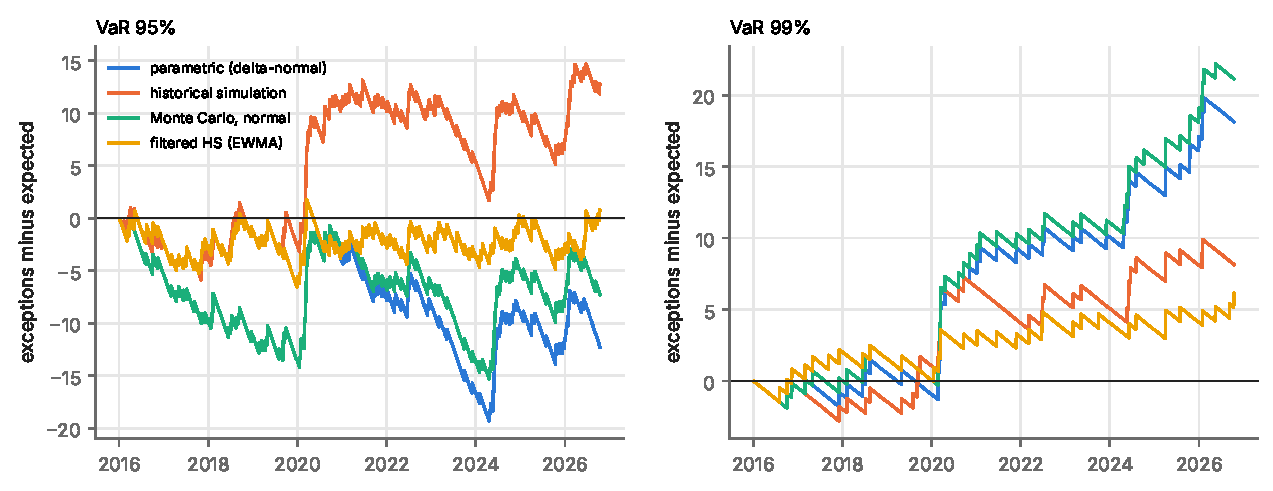
\includegraphics[width=\linewidth]{backtest_public.pdf}
  \caption{Cumulative number of VaR exceptions minus the expected number, 2016--2026. A correct VaR wanders around
    zero; a VaR that is too low drifts upwards; clustered exceptions appear as steps (March 2020, the copper and
    silver crashes of 2025--26).}
  \label{fig:backtest_public}
\end{figure}

Now the backtest separates the methods (\cref{tab:backtest_public,fig:backtest_public}):
\begin{itemize}
  \item \emph{Normal tails fail at 99\%.} The delta-normal and the normal Monte Carlo VaR are exceeded 45 and 48
    times instead of 27, Kupiec $p = 0.001$ and $0.0002$. At 95\% their counts are right (122 and 127 against 134):
    the normal distribution is adequate in the body of the distribution and wrong in the tail.
  \item \emph{Constant volatility gives clustered exceptions.} At 95\% the delta-normal VaR has the right number of
    exceptions, but they come in runs (Christoffersen $p = 0.03$): after March 2020 the 250-day volatility adapts too
    slowly, and the exceptions of a whole month count against the model.
  \item \emph{Historical simulation passes, with a lag.} It captures the empirical tail (35 exceptions at 99\%,
    $p = 0.13$) but adapts as slowly as its window: at 95\% it collected its surplus of exceptions in March 2020
    and again in early 2026.
  \item \emph{Filtered HS fits best.} Empirical tails rescaled by the EWMA volatility give 135 exceptions at 95\%
    (134 expected, $p = 0.95$) and 33 at 99\% ($p = 0.25$), with no sign of clustering at 95\%.
\end{itemize}
At 99\%, the independence test gives $p$ between 0.06 and 0.09 for all methods: some clustering remains, but about
30 exceptions are too few to say more. With 2686 test days, the Kupiec test detects a 99\% VaR with twice the nominal
exception rate in 99\% of the cases, against 13\% on the course data (\cref{tab:power_public}): the long backtest is
the one to trust.

\begin{table}[H]
  \centering\small
  \caption{Power of the Kupiec test (5\% significance): course backtest and public-data backtest.}
  \label{tab:power_public}
  \begin{tabular}{rrrr}
\toprule
VaR level & true exception rate & 132 days & 2686 days \\
\midrule
95\% & 7.5\% & 19\% & 100\% \\
95\% & 10.0\% & 57\% & 100\% \\
95\% & 15.0\% & 97\% & 100\% \\
99\% & 1.5\% & 5\% & 66\% \\
99\% & 2.0\% & 13\% & 99\% \\
99\% & 3.0\% & 36\% & 100\% \\
\bottomrule
\end{tabular}

\end{table}

% =====================================================================================================================
\section{Main changes with respect to the course notebook}

The notebook written for the exercise did not yet answer it. \Cref{tab:changes} lists the corrections.

\begin{table}[H]
  \centering\small
  \caption{Main changes with respect to the original notebook.}
  \label{tab:changes}
  \begin{tabular}{p{0.2\linewidth}p{0.36\linewidth}p{0.34\linewidth}}
    \toprule
    & course notebook & this version \\
    \midrule
    Alignment & returns of silver and EUR/USD paired by row position, not by date (correlation $-0.13$) & series
      aligned by date (correlation $+0.48$) \\
    Correlated shocks & Cholesky factor applied to draws already scaled by mean and volatility, volatility applied
      a second time when revaluing & Cholesky factor of the covariance applied to standard shocks \\
    Risk measure & 95th percentile of each factor's return separately; one simulated day revalued & quantile and
      tail mean of the loss of the position \\
    Units & 500 multiplied by a price per troy ounce & 500\,t $=$ \num{16.1e6} troy ounces \\
    Methods & Monte Carlo only & five methods, two levels, two horizons, ES \\
    Validation & none & backtest with Kupiec and Christoffersen tests, power analysis, on the course year and on eleven years of public data; tests on synthetic data \\
    \bottomrule
  \end{tabular}
\end{table}

% =====================================================================================================================
\section{Conclusions}

\begin{enumerate}
  \item The one-day VaR(95\%) of 500\,t of silver held in a euro balance sheet was EUR 8.3\,m in November 2023,
    \SI{2.5}{\percent} of its value. The positive correlation of silver with the euro is a natural hedge: without it
    the VaR would be \SI{18}{\percent} higher.
  \item For a book of silver and copper, the five methods give one-day 95\% VaRs between EUR 8.8 and 10.4\,m.
    Model choice matters in the tail: for the ten-day 99\% ES the estimates range from EUR 41 to 59\,m, and the
    methods that capture fat tails or changing volatility give the higher values.
  \item Diversification between the two commodities lowers the VaR by \SI{27}{\percent}.
  \item All methods pass the backtest on the course data, but half a year of backtest cannot tell good from mediocre
    models at the 99\% level. On eleven years of public data it can: normal tails underestimate the 99\% VaR
    (45--48 exceptions instead of 27), constant volatility produces clustered exceptions, and filtered historical
    simulation is the method to use for this book.
\end{enumerate}

\bibliographystyle{plainnat}
\bibliography{references}

\end{document}
